\documentclass[12pt]{report}
\usepackage[utf8]{inputenc}
\usepackage{amsmath}
\usepackage{amsfonts}
\usepackage{amssymb}
\usepackage[pdftex]{graphicx}
\usepackage{polski}

\usepackage{placeins}
\usepackage{epstopdf}
\usepackage{mathtools}
\usepackage{amsthm}
\usepackage{float}
\usepackage{tabularx}
\usepackage{titlesec}

\titleformat{\chapter}
{\Large\bfseries} % format
{}                % label
{0pt}             % sep
{\huge}           % before-code


\usepackage[left=2.50cm, right=2.50cm, top=2.50cm, bottom=2.50cm]{geometry}

\newcolumntype{C}[1]{>{\hsize=#1\hsize\centering\arraybackslash}X}
\newcolumntype{M}[1]{>{\centering\arraybackslash}m{#1}}

%opening
\title{\textbf{Sterowanie adaptacyjne i estymacja}}
\author{Maciej Cebula \\Kajetan Piertusa \\ Daniel Rubak}
\date{Kraków, 2017}
\begin{document}
	
%	\fancypagestyle{plain}
%	{
%		% Usuń nagłówek i stopkę
%		\fancyhf{}
%		% Usuń linie.
%		\renewcommand{\headrulewidth}{0pt}
%		\renewcommand{\footrulewidth}{0pt}
%	}

	
	\setcounter{tocdepth}{2}
	
	\maketitle
	\tableofcontents
	\clearpage
		
		\renewcommand{\tablename}{Tabela}
		\renewcommand{\figurename}{Rys.}
		
	\chapter{Wstęp}

\section{Cel zajęć}
Celem niniejszej pracy była analiza oraz dobór parametrów systemu adaptacyjnego w zależności od występujących w systemie zakłóceń oraz transmitancji obiektu, którym sterowano. Przyjęty model przedstawiono na rysunku \ref{model_systemu}.

\begin{figure}[h!]
	\centering
	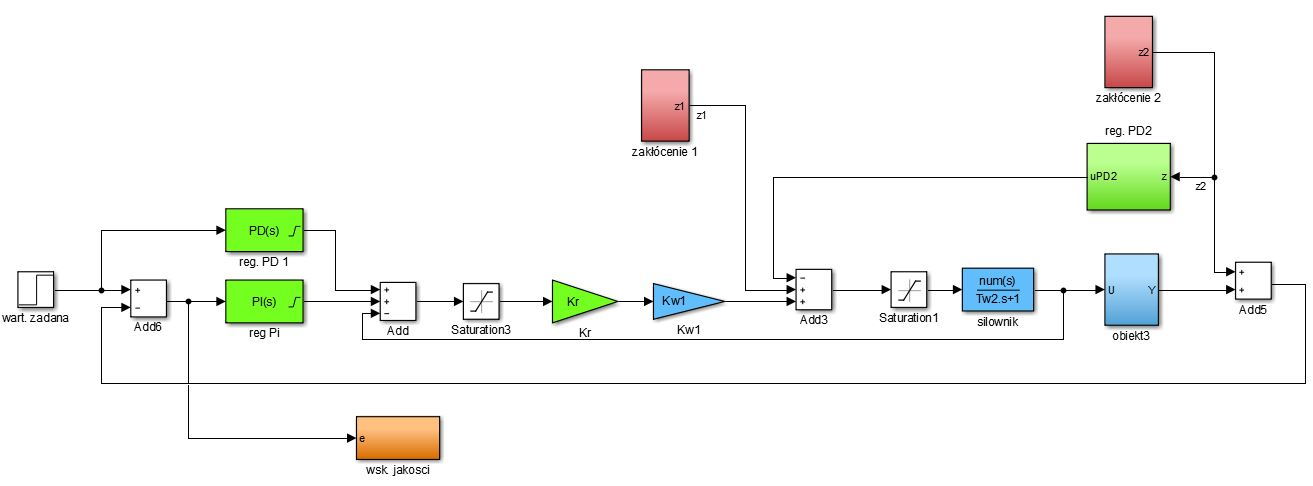
\includegraphics[scale = 0.6]{fig/model_systemu.png}
	\caption		
	{Model układu sterowania}
	\label{model_systemu}
\end{figure} 

Poszczególne regulatory znajdujące się na schemacie opisano następującymi wzorami: 
\begin{equation}\label{reg1}
PD_1 = \alpha_1+\beta_1 \cdot s
\end{equation}
\begin{equation}\label{reg2}
PD_2 = \alpha_2+\beta_2 \cdot s
\end{equation}\\
\begin{equation}\label{reg3}
PI = \gamma + \dfrac{\delta}{s}
\end{equation}
Element wykonawczy jest opisany za pomocą zależności:
\begin{equation}\label{actuator}
\dfrac{K_{w2}}{T_w s+T}
\end{equation}

Wartości parametrów $K_{w1}$, $K_{w2}$, $T_w$, $K_0$ potraktowano jako zadane. Przyjęto, iż testy zostaną przeprowadzone dla wartości zadanej $r$ dla pięciu różnych poziomów zmieniających się w zakresie $5-70^{\circ} C$. Zakłóceniem $z_1$ był niemierzalny skok $1(t)$, natomiast $z_2$ było mierzalnym skokiem $1(t)$.

W ramach projektu należało przeprowadzić optymalizację poszczególnych parametrów podanych powyżej regulatorów, tj. $\alpha_1$, $\beta_1$, $\alpha_2$, $\beta_2$, $\gamma$, $\delta$. Wskaźnikiem jakości, na mocy którego optymalizowano działanie całego układu, była całka z modułu uchybu:
\begin{equation}\label{wsk_jak}
J = \int |r-y| dt
\end{equation}. Ponadto przyjęto, iż oczekiwanym efektem optymalizacji będzie takie zachowanie układu, by bez względu na wartości zakłóceń $z_1$ i $z_2$, efekt nadążania i stabilizacji będzie najlepszy.


	\chapter{Optymalizacja}
 
\section{Wprowadzenie}

Do optymalizacji nastaw regulatorów wykorzystano skrypty zawarte w rozdziale \ref{implementacja}. Badania przeprowadzone zostały dla zestawu parametrów obiektu zaprezentowanego w tabeli \ref{tab_par}. Rząd obiektu jak i wartość zadana były zmiennymi parametrami o następujących wartościach: \\
$ n \in \{1,2,3\} $ - rząd obiektu, \\
$ z \in \{ 5,10,20,50,70\}$ - wartość zadana \\ 
%\subsection{Zestawy parametrów}
%W tabeli \ref{tab_par} zamieszczono przyjęte wartości parametrów opisujących obiekt regulacji.
\begin{table}[h!]
	\centering
	\caption{Zestawy parametrów dla których przeprowadzano optymalizację nastaw regulatorów.}
	\label{tab_par}
	\begin{tabular}{|c|c|} \hline
	Parametr & Wartość \\ \hline
	$K_{w1}$  & 10 \\ \hline
	$K_{w2}$  & 5 \\ \hline
	$T_{w2}$  & 0.1 \\ \hline
	$T_0$   & 1 \\ \hline
	$K_0$   & 10 \\ \hline
	$\tau$ & 1 \\ \hline
	\end{tabular}
\end{table}
\FloatBarrier

\section{Optymalizacja nastaw regulatorów}
Dla kolejnych zestawów parametrów opisujących system przeprowadzano procedurę optymalizacji nastaw regulatorów minimalizując wska\'znik jakości opisany zależnością \ref{wsk_jak}. Proces optymalizacji przeprowadzany był dla różnych wartości zadanych w obecności znanego zakłócenia $z_2$ (zakłócenie skokowo zmieniające swoją wartość) oraz nieznanego zakłócenia $z_1$. Przebiegi owych zakłóceń przedstawiono na rysunku \ref{fig_zaklocenia}. 

\begin{figure}[h!]
	\centering
	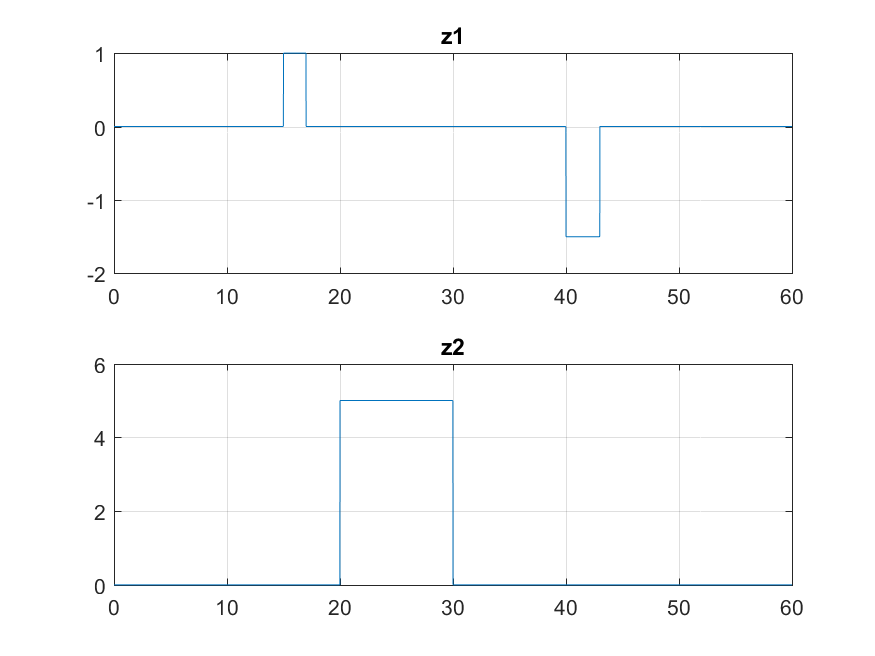
\includegraphics[scale = 0.8]{fig/Z1_New_Signal_1/fig3_1_5.png}
	\caption		
	{Zakłócenia.}
	\label{fig_zaklocenia}
\end{figure} 

Dla przedstawionych powyżej przebiegów zakłóceń przeprowadzono optymalizację a otrzymane nastawy dla poszczególnych obiektów zamieszczono w tabelach \ref{par_reg_zes1} - \ref{par_reg_zes3}. 

\begin{table}[h!]
	\centering
	\caption{Parametry regulatorów dla obiektu pierwszego rzędu.}
	\label{par_reg_zes1}
	\begin{tabular}{|c|c|c|c|c|c|c|c|}
		\hline
		\multicolumn{1}{|l|}{\begin{tabular}[c]{@{}l@{}}Parametr regulatora\textbackslash\\ Wart. zadana\end{tabular}} & $P1$ & $D1$ & $P2$ & $D2$ & $P3$ & $I3$ & $Kr$ \\ \hline
		5 & 0,1583 & 0,0000 & 0,3902 & 503,9885 & 0,0565 & 0,0393 & 1,3697 \\ \hline
		10 & 0,0875 & 0,0245 & 0,2230 & 0,3092 & 0,0454 & 0,0000 & 0,5617 \\ \hline
		20 & 0,1037 & 45,9950 & 0,4478 & 310,6393 & 0,0336 & 0,0000 & 0,5367 \\ \hline
		50 & 0,0800 & 12,6157 & 0,0000 & 4,8505 & 0,0326 & 0,0164 & 0,5671 \\ \hline
		70 & 0,0571 & 3,3536 & 0,0000 & 213,3236 & 0,0496 & 0,0331 & 0,5549 \\ \hline
	\end{tabular}
\end{table}

\begin{table}[h!]
	\centering
	\caption{Parametry regulatorów dla obiektu drugiego rzędu.}
	\label{par_reg_zes2}
	\begin{tabular}{|c|c|c|c|c|c|c|c|}
		\hline
		\multicolumn{1}{|l|}{\begin{tabular}[c]{@{}l@{}}Parametr regulatora\textbackslash\\ Wart. zadana\end{tabular}} & $P1$ & $D1$ & $P2$ & $D2$ & $P3$ & $I3$ & $Kr$ \\ \hline
		5 & 0,1036 & 0,3042 & 0,5315 & 73,9744 & 0,0442 & 0,0000 & 0,5367 \\ \hline
		10 & 0,1037 & 0,7795 & 0,5391 & 1,5989 & 0,0353 & 0,0000 & 0,5367 \\ \hline
		20 & 0,1031 & 17,033 & 0,5250 & 0,2906 & 0,0238 & 0,0000 & 0,5390 \\ \hline
		50 & 0,0800 & 0,1205 & 0,3564 & 37,7697 & 0,0509 & 0,0112 & 0,5420 \\ \hline
		70 & 0,0571 & 728,1221 & 0,2330 & 18,4368 & 0,0475 & 0,0222 & 0,5378 \\ \hline
	\end{tabular}
\end{table}

\begin{table}[h!]
	\centering
	\caption{Parametry regulatorów dla obiektu trzeciego rzędu.}
	\label{par_reg_zes3}
	\begin{tabular}{|c|c|c|c|c|c|c|c|}
		\hline
		\multicolumn{1}{|l|}{\begin{tabular}[c]{@{}l@{}}Parametr regulatora\textbackslash\\ Wart. zadana\end{tabular}} & $P1$ & $D1$ & $P2$ & $D2$ & $P3$ & $I3$ & $Kr$ \\ \hline
		5 & 0,1800 & 0,1319 & 1106,0058 & 0,4266 & 0,0143 & 0,0000 & 1,2768 \\ \hline
		10 & 0,1017 & 0,9193 & 0,4593 & 0,1072 & 0,0345 & 0,0000 & 0,5416 \\ \hline
		20 & 0,1026 & 3,2520 & 0,4596 & 123,9292 & 0,0283 & 0,0000 & 0,5438 \\ \hline
		50 & 0,0800 & 7164,0578 & 0,3120 & 6756,3846 & 0,0303 & 0,0084 & 0,5445 \\ \hline
		70 & 0,0571 & 29629,2945 & 0,1710 & 400,4956 & 0,0414 & 0,0153 & 0,5448 \\ \hline
	\end{tabular}
\end{table}

W tabeli \ref{wsk_jakosci_tab} przedstawiono wartości wskaźnika jakości dla wszystkich przeprowadzonych symulacji.

\begin{table}[h!]
	\centering
	\caption{Wartości wska\'znika jakości dla różnych wartości zadanych i różnych zestawów parametrów opisujących system.}
	\label{wsk_jakosci_tab}
	\begin{tabular}{|c|c|c|c|}
		\hline
		\multicolumn{1}{|l|}{\begin{tabular}[c]{@{}l@{}}Nr zestawu\textbackslash\\ Wart. zadana\end{tabular}} & 1 & 2 & 3 \\ \hline
		5 & 33,0087 & 43,1130 & 54,9063 \\ \hline
		10 & 38,7111 & 52,7556 & 70,6049 \\ \hline
		20 & 64,0122 & 71,5313 & 100,7350 \\ \hline
		50 & 94,3375 & 158,9382 & 195,2509 \\ \hline
		70 & 131,8947 & 198,0144 & 272,9748 \\ \hline
	\end{tabular}
\end{table}

\FloatBarrier
Na rysunkach \ref{wykres_1} - \ref{wykres_4} przedstawiono przykładowe przebiegi zawierające odpowiedzi obiektów dla różnych wartości zadanych.

\begin{figure}[h!]
	\centering
	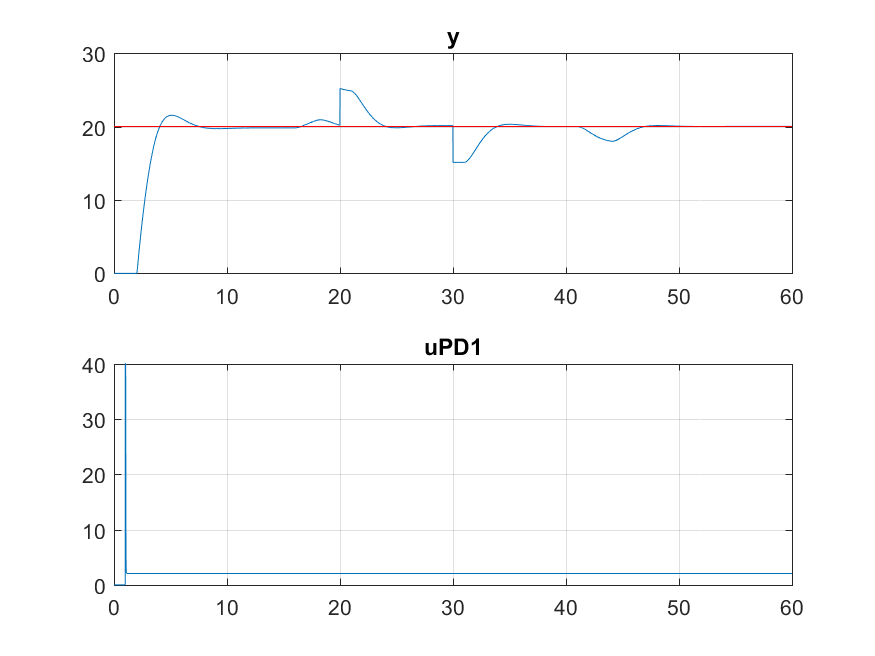
\includegraphics[scale = 0.8]{fig/Z1_New_Signal_1/fig1_2_20.png}
	\caption		
	{Odpowiedź obiektu drugiego rzędu, r = 20}
	\label{wykres_1}
\end{figure} 

\begin{figure}[h!]
	\centering
	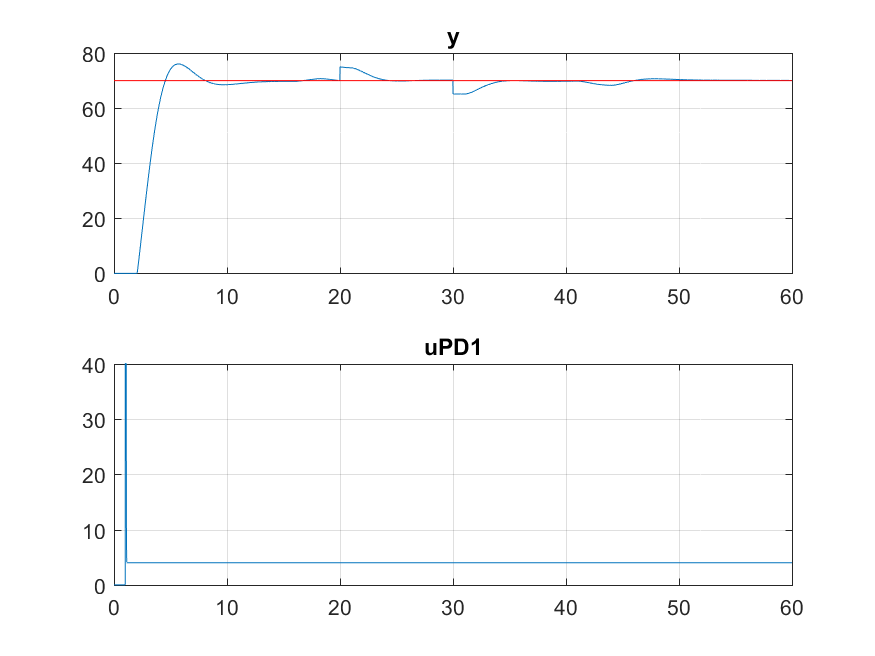
\includegraphics[scale = 0.8]{fig/Z1_New_Signal_1/fig1_2_70.png}
	\caption		
	{Odpowiedź obiektu drugiego rzędu, r = 70}
	\label{wykres_2}
\end{figure} 

\begin{figure}[h!]
	\centering
	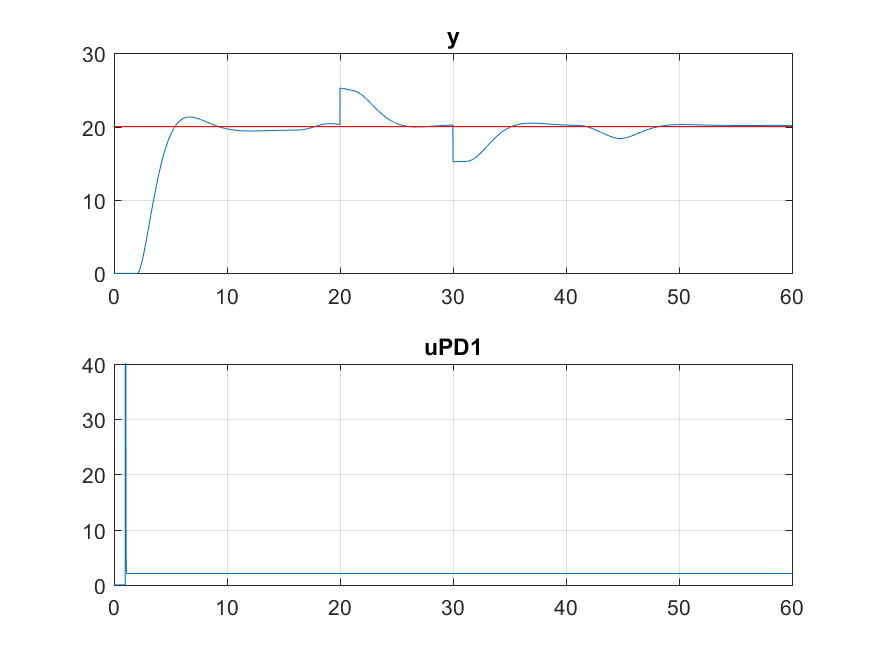
\includegraphics[scale = 0.8]{fig/Z1_New_Signal_1/fig1_3_20.png}
	\caption		
	{Odpowiedź obiektu trzeciego rzędu, r = 20}
	\label{wykres_3}
\end{figure} 

\begin{figure}[h!]
	\centering
	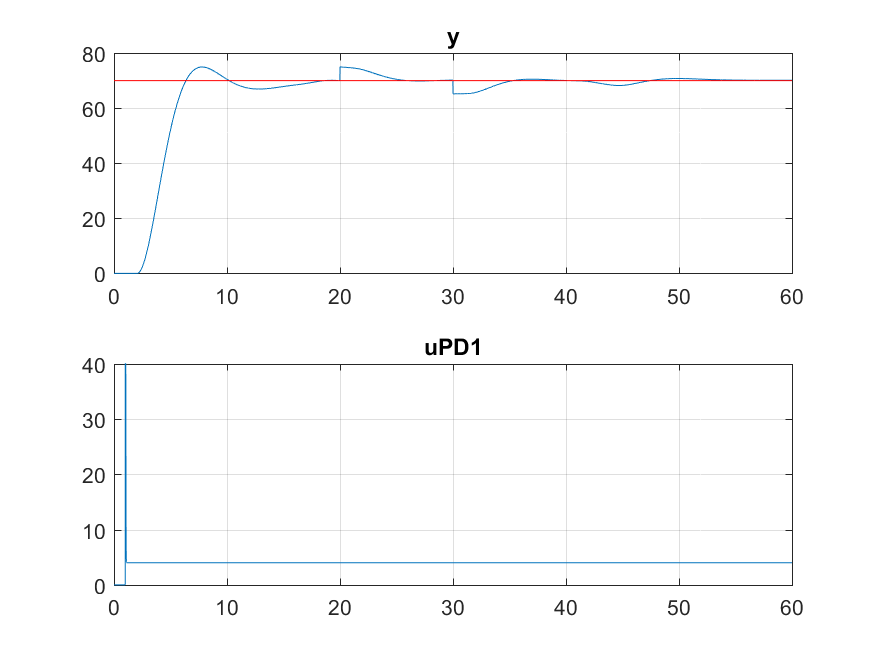
\includegraphics[scale = 0.8]{fig/Z1_New_Signal_1/fig1_3_70.png}
	\caption		
	{Odpowiedź obiektu trzeciego rzędu, r = 70}
	\label{wykres_4}
\end{figure}

\begin{table}[h!]
	\centering
	\caption{Wartości nastaw regulatorów oraz wska\'znika jakości dla różnych wartości zadanych i różnych zestawów zakłóceń.}
	\label{bez_feedforward_tab}
	\begin{tabular}{|c|c|c|c|c|c|c|}
		\hline
		r & z1 & z2& P3 & I3 & Kr & J \\ \hline
		20 & Nieaktywne & Nieaktywne & 0,1725 & 0,0742 & 0,0093 & 62,92709248 \\ \hline
		0 & Nieaktywne & Aktywne & 5,4818 & 2,3818 & 0,0003 & 30,5386 \\ \hline
		0 & Aktywne & Aktywne & 1,7981 & 0,3955 & 0,0012 & 309,0387 \\ \hline
	\end{tabular}
\end{table}

\begin{figure}[h!]
	\centering
	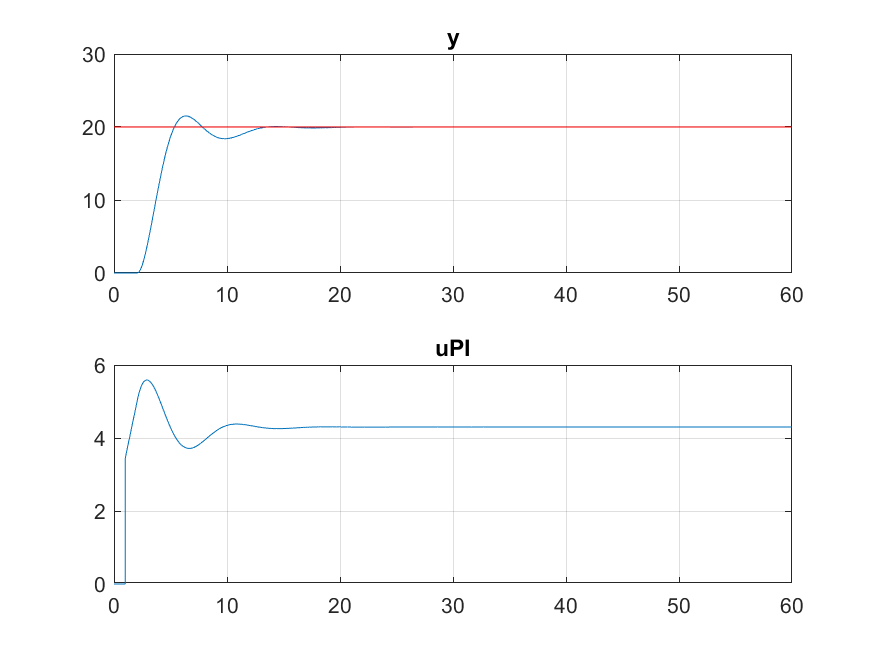
\includegraphics[scale = 0.8]{fig/bezFeedforward/fig1_2_20_bezZaklocen.png}
	\caption		
	{Odpowiedź obiektu drugiego rzędu bez regulatora feedforward, r = 20}
	\label{wykres_5}
\end{figure} 

\begin{figure}[h!]
	\centering
	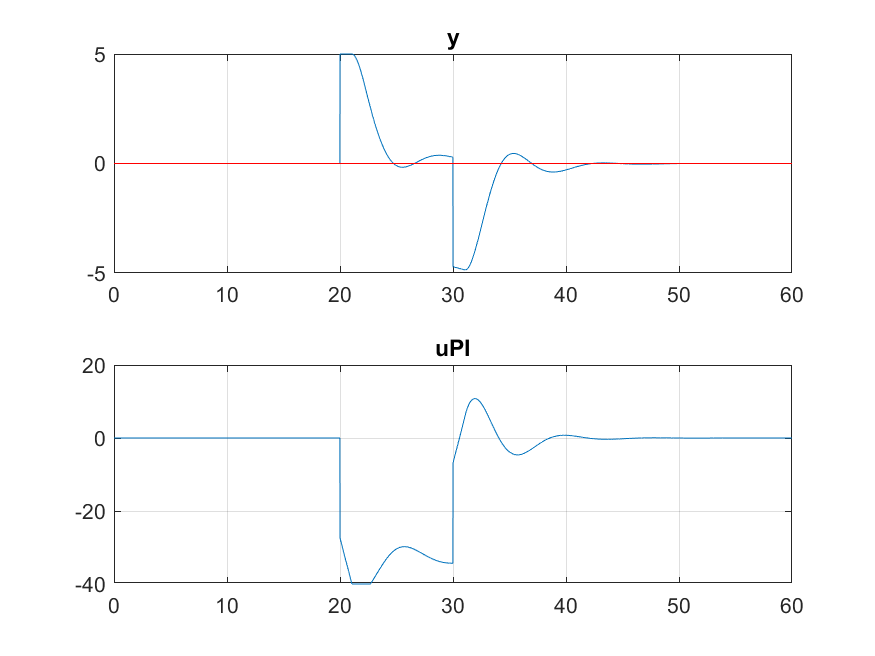
\includegraphics[scale = 0.8]{fig/bezFeedforward/fig1_2_0_z2.png}
	\caption		
	{Odpowiedź obiektu drugiego rzędu bez regulatora feedforward, r = 0, aktywne zakłócenie z2}
	\label{wykres_6}
\end{figure}

\begin{figure}[h!]
	\centering
	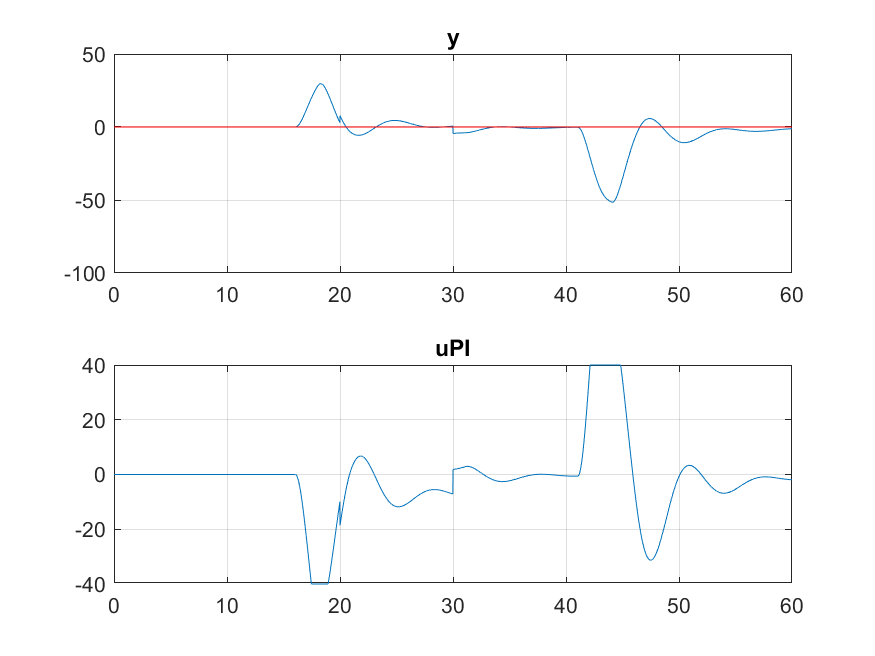
\includegraphics[scale = 0.8]{fig/bezFeedforward/fig1_2_0_z1z2.png}
	\caption		
	{Odpowiedź obiektu drugiego rzędu bez regulatora feedforward, r = 0, aktywne oba zakłócenia}
	\label{wykres_7}
\end{figure}

	
	\begin{thebibliography}{}
	
	%przykład 
	
%	\bibitem{pauluk 1}Pauluk, M.: 
%	\emph{Model matematyczny trójwymiarowej suwnicy.} W: \textbf{Automatyka} 2002 tom 6 s. 69-102, ISSN: 1429-3447
%

\bibitem{byrski}
  Witold Byrski,
  \emph{Obserwacja i sterowanie w systemach dynamicznych}.
  Wydawnictwa AGH, Kraków, 2007.	
	
\end{thebibliography}
	
\end{document}